"An introduction to variational quantum algorithms for combinatorial optimization problems" \cite{grange2023introduction}

\vspace{10pt}

Variational Quantum Algorithms are heuristic algorithms that alternate between a quantum circuit and a classical optimizer. They tackle optimization problems of the form
\begin{equation}
    \min _{x \in\{0,1\}^n} f(x), \tag{1}
\end{equation}
where $f$ is any function defined on $\{0,1\}^n$. 

\section{Basics of Quantum Computing for Combinatorial Optimization}

\subsection{Quantum Bits \& Quantum Gates}

\begin{definition}[Canonical basis]
    The canonical basis of an $n$-qubit state is the set
\begin{equation}
    \mathcal{CB}_{n}=
\left\{\bigotimes_{k=1}^{n}\left|i^{(k)}\right\rangle,\left(i^{(1)}, \ldots, i^{(n)}\right) \in\{0,1\}^{n}\right\}
\end{equation}
where $i^{(k)}$ represents the state of the $k$-th qubit and $\otimes$ is the tensor product. For more readability, we omit to write the tensor product between qubits, i.e.,
\begin{equation}
    \mathcal{C B}_{n}=\left\{|i\rangle, i \in\{0,1\}^{n}\right\}.
\end{equation}
\end{definition}

The canonical basis is the set of all possible combinations of tensor products of $n$ one-qubit basis states, $|0\rangle$ and $|1\rangle$. Thus, in the matrix representation, each canonical basis state is a column vector of $2^{n}$ components with one component equal to 1 and the rest equal to 0. It directly results that the size of the canonical basis of an $n$-qubit state is $2^{n}$. 

% reversible %可逆的,相当于数学用语inverse, invertible

% $\left|\Phi^{+}\right\rangle=\frac{|00\rangle+|11\rangle}{\sqrt{2}}$

\subsection{Quantum Circuits}

In the circuit representation, qubits are numbered \textit{in ascending order from top to bottom} which is important for the tensor product circuit representation that follows. % 注意从电路图上看,composition的顺序是从左边到右边,而tensor的顺序是从上边到下边。这两类操作都是不可交换的操作,所以顺序很重要。

\subsubsection{Manipulate Quantum Gates to Build Other Quantum Gates}

We can manipulate quantum gates to build other quantum gates in two different ways. 
\begin{enumerate}
    \item The first one is the \textit{composition}. The composition of gates only operates between gates acting on the same qubits. 
\begin{figure}[h]
    \centering
    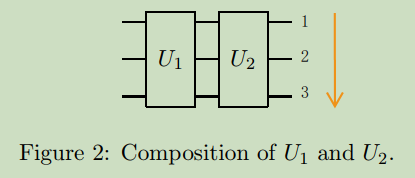
\includegraphics[width=0.5\linewidth]{Images/grange2023-1.png}
\end{figure}
    \item The other one is the \textit{tensor product}. The tensor product of gates can operates between gates acting on different qubits. Suppose $U_{1} \in \mathcal{M}_{2^{k}}(\mathbb{C})$ applies on the first $k$ qubits and $U_{2} \in \mathcal{M}_{2^{k^{\prime}}}(\mathbb{C})$ applies on the $k^{\prime}$ following ones. Their tensor product is the application of $U_{1}$ and $U_{2}$ on respective qubits in parallel. The matrix representation of this tensor product is $U_{1} \otimes U_{2}$. 
\begin{figure}[h]
    \centering
    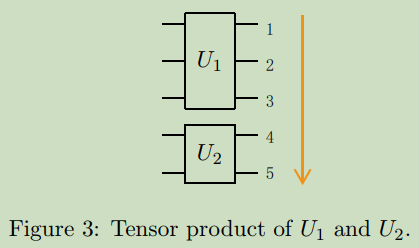
\includegraphics[width=0.5\linewidth]{Images/grange2023-2.png}
\end{figure}
\end{enumerate}
One readily verifies that both composition and tensor product transform unitary matrices into a resulting unitary matrix.

Notice that when we apply a quantum gate on $k$ qubits of an $n$-qubit system, it supposes that we apply identity gate $I$ on the qubits not concerned. 

\begin{example}
For instance, let us consider a 3-qubit system on which we apply $U \in \mathcal{M}_{2}(\mathbb{C})$ on qubit number 2. The matrix representation of the resulting 3-qubit gate is $I \otimes U \otimes I$, and its circuit representation is illustrated on Fig.4, where the application of $I$ is usually replaced by a simple wire.
\begin{figure}[h]
    \centering
    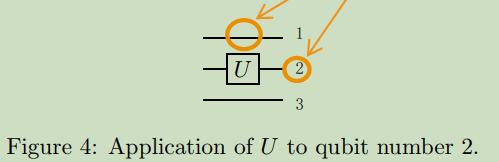
\includegraphics[width=0.5\linewidth]{Images/grange2023-3.png}
\end{figure}
\end{example}

\subsubsection{What is a Quantum Algorithm?}

Throughout, we consider that \textit{a quantum algorithm is a quantum circuit acting on $n$ qubits, that is, a sequence of quantum gates' compositions and/or tensor products. } % 概括得挺好

These quantum gates can be $k$-qubit gates, for $k \in[n]$. % k是小于等于n的整数。相对于很大n,当k足够小时,k-qubit gates 就可以称之为 small gates。

However, quantum gates involving many qubits are typically not implementable natively on quantum computers and need to be decomposed into smaller and simpler gates. This set of small gates can be considered as the quantum counterpart of the elementary logic gates used in classical circuit computing to assess \textit{the circuit complexity} of a classical algorithm. % 也就是说电路的复杂度可以由构成其的基础gates的个数来做衡量,这一想法是来自于经典电路的。

Thus, an $n$-qubit quantum algorithm is described by a unitary matrix in $\mathcal{M}_{2^{n}}(\mathbb{C})$, and we decompose it as a sequence of universal gates to obtain the \textit{complexity of the quantum algorithm}. % 也就是说量子电路的复杂度可以由构成其的基础量子gates的个数来做衡量

\subsubsection{Universal Gates}

\begin{definition}[Set of universal gates]
    A set of quantum gates PU is \textit{universal} if we can decompose any $n$-qubit quantum gate through a circuit composed solely of the gates in PU.
\end{definition}

\begin{remark}
\begin{itemize}
    \item In definition above, we implicitly allow PU to be a set of infinite elements (countable or uncountable). Of course, we want PU to be small as soon as possible.
    \item In definition above, the word "composed" contains both the composition operations and tensor product operations.
    \item Note that this "decompose" is exact decomposition, and there no error.
\end{itemize}
\end{remark}

Fortunately, there exist different universal sets of quantum gates. We introduce below such a set formed of four types of gates. 

\begin{example}[Some important small gates]
First, we consider the three following families of one-qubit gates, each of which is parametrized by a real number $\theta \in \mathbb{R}$:
\begin{align}
& R_{X}(\theta)=\left(\begin{array}{cc}
\cos \frac{\theta}{2} & -i \sin \frac{\theta}{2} \\
-i \sin \frac{\theta}{2} & \cos \frac{\theta}{2}
\end{array}\right)  \tag{5}\\
& R_{Y}(\theta)=\left(\begin{array}{cc}
\cos \frac{\theta}{2} & -\sin \frac{\theta}{2} \\
\sin \frac{\theta}{2} & \cos \frac{\theta}{2}
\end{array}\right)  \tag{6}\\
& R_{Z}(\theta)=\left(\begin{array}{cc}
e^{-i \frac{\theta}{2}} & 0 \\
0 & e^{i \frac{\theta}{2}}
\end{array}\right) \tag{7}
\end{align}
Second, we consider the two-qubit gate CX (or, CNOT, Controlled Not, Controlled X gate):
\begin{equation}
    C X=\left(\begin{array}{llll}
1 & 0 & 0 & 0  \tag{8}\\
0 & 1 & 0 & 0 \\
0 & 0 & 0 & 1 \\
0 & 0 & 1 & 0
\end{array}\right)
\end{equation}
In other words, we can define $C X$ on the canonical basis as
\begin{equation}
    C X|a, b\rangle=|a, b \oplus a\rangle
\end{equation}
for $a, b \in\{0,1\}$, where $\oplus$ is the addition modulo 2 .
\end{example}

\begin{remark}[Notation on gates indexes]
Henceforth, we use the notation $R_{X, i}$ for the application of $R_{X}$ on qubit $i$ (and the application of identity matrix on the remaining qubits). We do the same with $R_{Y, i}$ and $R_{Z, i}$. 
% 这一中比较偷懒的写法:$R_{X, i}$,可以用来表示一个非常大的gates,但其中只有第i个qubit是受到非平凡的$R_{X}$的操作。这类写法在其他文献中也经常使用。
We note $C X_{i, j}$ the application of $C X$ gate to qubits $i$ and $j$: $X$ is applied to qubit $j$ if and only if qubit $i$ is in state $|1\rangle$.
% 明确标记控制位i和操作位j也是CX门常见写法。但有时不同文献会有细微差别,要注意别混淆。
\end{remark}

\begin{theorem}[Universal gates \cite{nielsen2010quantum}]
We claim that
\begin{itemize}
    \item The set of all one-qubit gates and the $C X$ gate is universal.
    \item Any one-qubit gate is the composition of rotation gates (5)-(7).
    \item Thus, the set 
\begin{equation}
    P U=\left\{R_{X}(\alpha), R_{Y}(\beta), R_{Z}(\gamma), C X: \alpha, \beta, \gamma \in \mathbb{R}\right\}
\end{equation}
is also universal.
\end{itemize}
\end{theorem}

In comparison, the sets of gates $\{N A N D\},\{N O R\},\{N O T, A N D\}$ and $\{N O T, O R\}$ are universal for classical computation. \todo{Need proof.} Indeed, we can compute any arbitrary classical function with them. % 这一部分知识是传统计算科学里出现的证明,未来有时间好好研究一下。

In view of the above, we typically consider that the quantum counterpart of the classical number of elementary operations is the number of universal gates used to decompose the circuit. Of course, this decomposition depends on the set of universal gates $P U$ considered, but the number of gates required is the same with any set, modulo a multiplicative constant. 

% Thereafter, we only consider the set $P U$ defined in Theorem 13. This choice is motivated by the algorithms we study in this paper, as it will be convenient to express them with this set. 

Furthermore, if we consider the family of circuits $\left(\mathcal{C}_{n}\right)_{n \in \mathbb{N}}$ where $\mathcal{C}_{n}$ is a circuit on $n$ qubits and is decomposed on $\mathcal{O}(\operatorname{poly}(n))$ universal quantum gates, then this family is said to be \textit{efficient}.

\subsection{Non-classical Behaviors} % 确实,前面几节没有让人感觉奇怪的设定。作者把量子特有的设定放在一起,以区别经典行为。这一思路值得借鉴。

The quantum algorithms rely on three characteristics of quantum states with no classical equivalent: measurement, superposition, and entanglement.

\subsubsection{Measurement} %该论文的测量介绍,把很艰难晦涩的测量,用短短的语言就清晰地刻画了。很值得学习。他不涉及各种可观测量,投影算子,POVM等复杂概念。

We need to measure a quantum state $|\psi\rangle$ to get information from it; otherwise, no information is accessible.
Moreover, it only extracts partial information from the quantum state at once measurement: the single measurement output of  $|\psi\rangle$ is a bitstring\footnote{$n$-bitstring is the element of $\{0,1\}^{n}$}.

\begin{definition}[Measurement]
    In the gate-based quantum model, the measurement $\mathcal{M}$ of an $n$-qubit state $|\psi\rangle=\sum_{i \in\{0,1\}^{n}} \psi_{i}|i\rangle$ outputs the $n$-bitstring $i$ with probability $\left|\psi_{i}\right|^{2}$. After having been measured, state $|\psi\rangle$ no longer exists: it has been replaced by the state $|i\rangle$.
\end{definition}

\begin{example}
    For example, measuring qubit $|q\rangle=q_{0}|0\rangle+q_{1}|1\rangle$ outputs 0 with probability $\left|q_{0}\right|^{2}$ and 1 with probability $\left|q_{1}\right|^{2}$, and changes the state $|q\rangle$ to $|0\rangle$ and $|1\rangle$, respectively.  % 这个例子值得玩味的点是,我们测量得到的结果outcome是label(用bitstring表示),而原量子态坍缩成对应的label的basis state。所以,不应该说,测量得到的结果就是basis state自身。
\end{example}

Some points:
\begin{itemize}
    \item A measurement appears as a loss of information. Indeed, we describe an $n$-qubit state by $2^{n}$ normalized complex coefficients, but we only extract an $n$-bitstring after measuring it.
    \item The perfect knowledge of the probabilities representing a given quantum state $|\psi\rangle$, namely, the square module of each of its coordinates 
    \begin{equation}
    \left(\left|\psi_{i}\right|^{2}\right)_{i \in\{0,1\}^{n}} \in[0,1]^{2^{n}},
\end{equation}
can be obtained \textit{only if we measure $|\psi\rangle$ an infinite number of times.} Notice that it requires resetting state $|\psi\rangle$ after each measurement.
    \item Note that we never get the exact complex numbers $\psi_{i}$, instead of, their squared module $\left|\psi_{i}\right|^{2}$ at most.
    \item Different qubit state might have the same probabilities representing.
\end{itemize}

In reality we are limited to approximating a given quantum state through sampling. In particular, if $|\psi\rangle$ is the result of an algorithm, this means we have to repeat the same algorithm for every measurement of $|\psi\rangle$ we wish to perform.

\subsubsection{Superposition}

\begin{definition}[Superposition]
    A quantum state $|\psi\rangle$ is said in superposition if $|\psi\rangle=$ $\sum_{i \in\{0,1\}^{n}} \psi_{i}|i\rangle$ where there are \textit{at least two terms }with non-zero coefficients in the sum. Equivalently, a quantum state that is not a basis state is in superposition.
\end{definition}

\begin{remark}
    \begin{itemize}
    \item A quantum state is in superposition. = A quantum state is superposed.
    \item A quantum stated superposed is $\dots$
    \end{itemize}
\end{remark}

The Hadamard gate $H=\frac{1}{\sqrt{2}}\left(\begin{array}{cc}1 & 1 \\ 1 & -1\end{array}\right)$ is essential in quantum computing because it creates superposition starting from a basis state. We obtain the state $|+\rangle$, respectively $|-\rangle$, by applying $H$ on $|0\rangle$, respectively $|1\rangle:$
\begin{equation}
\begin{aligned}
& H|0\rangle=\frac{|0\rangle+|1\rangle}{\sqrt{2}}=:|+\rangle \\
& H|1\rangle=\frac{|0\rangle-|1\rangle}{\sqrt{2}}=:|-\rangle
\end{aligned}
\end{equation}
The two states $|+\rangle$ and $|-\rangle$ are in uniform superposition because both have the same probability of being measured as 0 or 1.

\begin{definition}[uniformly superposition]
    In general, an $n$-qubit state is in uniformly superposition if it is equal to 
\begin{equation}
    \frac{1}{\sqrt{2^{n}}} \sum_{j \in\{0,1\}^{n}} e^{i \alpha_{j}}|j\rangle,
\end{equation}
with $\alpha_{j} \in\left[0,2 \pi\left[, \forall j \in\{0,1\}^{n}\right.\right.$. % 注意,uniform的含义不是非要各个系数自身相等,而是他们的modulus相等。下面的$|+\rangle^{\otimes n}$ 提供一种各个系数自身相等的特殊情况。
In what follows, we shall often use the following uniformly superposed $n$-qubit state 
\begin{equation}
    |+\rangle^{\otimes n}=\frac{1}{\sqrt{2^{n}}} \sum_{i \in\{0,1\}^{n}}|i\rangle.
\end{equation}
\end{definition}

\begin{remark} 
Some points in definition above:
    \begin{itemize}
    \item $[0,2 \pi[$ means $[0,2 \pi)$.
    \item Sometimes, we need carefully distinguish "index $i$ " with "pure imaginary number $i$". 
    \end{itemize}
\end{remark}

When applying the tensor product of $n$ Hadamard gates, each applied to a qubit initially in state $|0\rangle$, specifically
\begin{equation}
    H^{\otimes n}|0\rangle^{\otimes n}=\bigotimes_{i=1}^{n} H|0\rangle=\bigotimes_{i=1}^{n}\left(\frac{|0\rangle+|1\rangle}{\sqrt{2}}\right)=\frac{1}{\sqrt{2^{n}}} \sum_{i \in\{0,1\}^{n}}|i\rangle=|+\rangle^{\otimes n}. \tag{9}
\end{equation}
In the left first equality, we used the following relation
\begin{equation}
    (A \otimes B)(C \otimes D)=(A C \otimes B D).
\end{equation}
Equation (9) illustrates the potential benefit of quantum circuits: applying $\mathcal{O}(n)$ universal one-qubit gates impacts the exponentially many coefficients of $|\psi\rangle$. Indeed, one readily verifies that 
\begin{equation}
    H=R_{X}(\pi) R_{Y}\left(\frac{\pi}{2}\right)
\end{equation}
modulo a global phase, so $H^{\otimes n}$ amounts to applying $2 n$ universal one-qubit gates.

\begin{remark}
    Two quantum states $|\psi\rangle$ and $\left|\psi^{\prime}\right\rangle=e^{i \alpha}|\psi\rangle$, with $\alpha \in[0,2 \pi[$, that only differ by a global phase are indiscernible by measurement. Thus, \textit{we do not consider global phase of quantum states nor quantum gates.} % 无论是gate还是state,如果只相差一个modulu 为1的复数因子,我们都不区分它们,而把他们当作一个东西。
\end{remark}

\subsubsection{Entanglement}

Entanglement has the peculiar and helpful property that we can apply a circuit only on a part of the $n$-qubit system, and as a result, the whole system is affected.

\begin{definition}[Product state]
    An $n$-qubit state is a product state if it is the tensor product of $n$ one-qubit states. In other words, an $n$-qubit state $|\psi\rangle$ is a product state if it exists $2 n$ complex coefficients $\left(q_{0}^{(j)}, q_{1}^{(j)}\right)_{j \in[n]}$ such that
\begin{equation}
    |\psi\rangle=\bigotimes_{j=1}^{n}\left(q_{0}^{(j)}|0\rangle+q_{1}^{(j)}|1\rangle\right), \text { with }\left|q_{0}^{(j)}\right|^{2}+\left|q_{1}^{(j)}\right|^{2}=1, \forall j \in[n].
\end{equation}
Thus, each state of a qubit that composes $|\psi\rangle$ can be described independently of the states of the other.
\end{definition}

\begin{definition}[Entangled state]
    An $n$-qubit state $|\psi\rangle=\sum_{i \in\{0,1\}^{n}} \psi_{i}|i\rangle$ is entangled if the numerical values of its coordinates $\left(\psi_{i}\right)_{i \in\{0,1\}^{n}} \in \mathbb{C}^{2^{n}}$ admit no solution $\left(q_{0}^{(j)}, q_{1}^{(j)}\right)_{j \in[n]} \in \mathbb{C}^{2 n}$ to the system
\begin{equation}
    \left\{\begin{array}{l}
\sum_{i \in\{0,1\}^{n}} \psi_{i}|i\rangle=\bigotimes_{j=1}^{n}\left(q_{0}^{(j)}|0\rangle+q_{1}^{(j)}|1\rangle\right) \\
\left|q_{0}^{(j)}\right|^{2}+\left|q_{1}^{(j)}\right|^{2}=1, \forall j \in [n]
\end{array}\right.
\end{equation}

\end{definition}

If an $n$-qubit state is not a product state, it is an entangled state. Operations performed on some coordinates of the entangled state can affect the other coordinates without direct operations on them.

\begin{remark}
    \begin{itemize}
    \item Each quantum state is either a product state or an entangled state.
    \item Each quantum state is either a basis state or a superposed state.
    \item There is a difference between superposition and entanglement, but there are some implication relation between those concepts, see next figure. % 但又有一些关联
\begin{figure}[h]
    \centering
    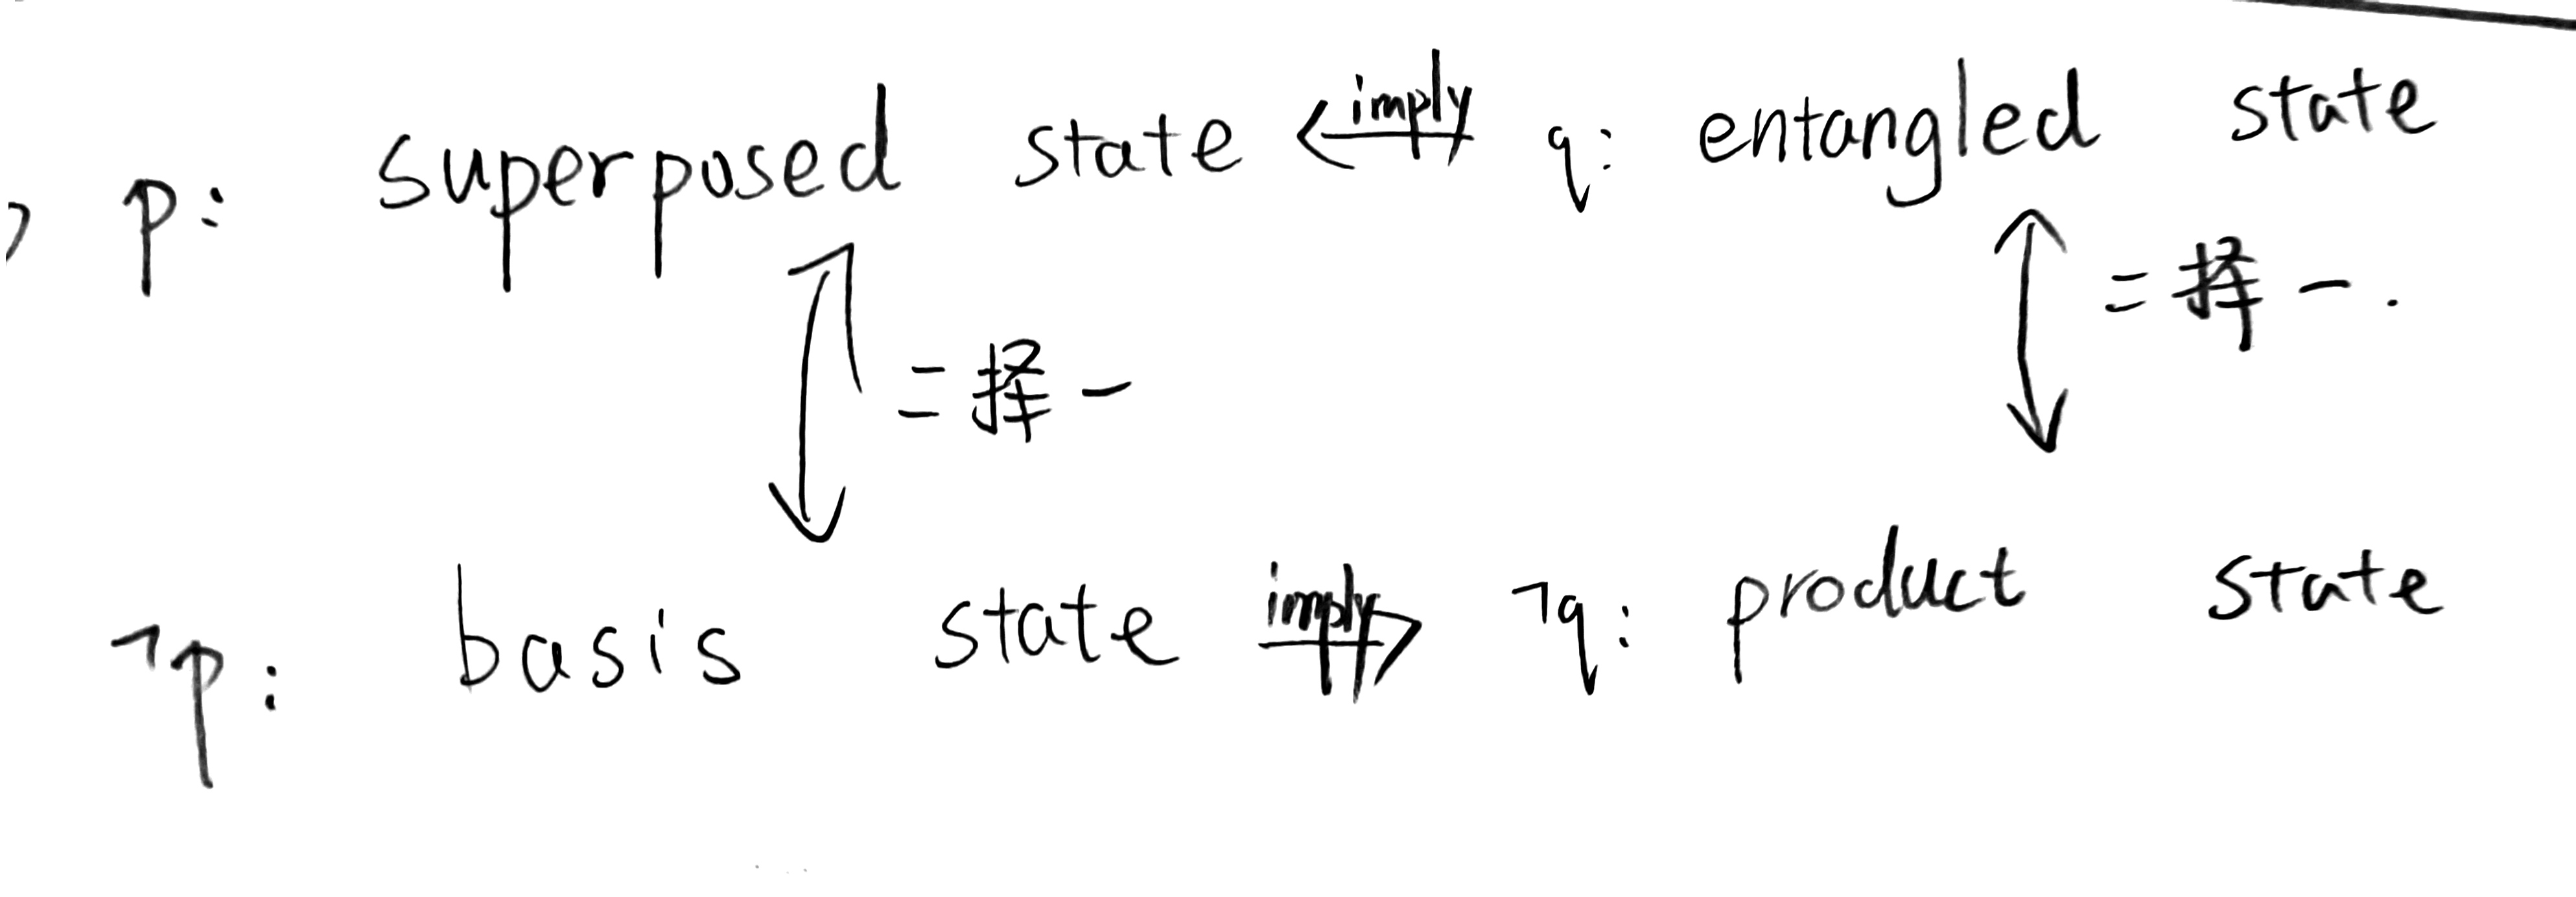
\includegraphics[width=0.75\linewidth]{Images/relation-superposed-entangled.jpg}
\end{figure}
    \item Notice that when an $n$-qubit system is entangled, it makes no sense to speak about qubit number $k \in[n]$ because isolated qubits are not defined. 
    \end{itemize}
\end{remark}

\section{Variational Quantum Algorithms for Optimization}

Some of the quantum algorithms that tackle combinatorial optimization problems are Variational\footnote{The word "variational" does not have that mathematical meaning.} Quantum Algorithms (VQAs). They are hybrid algorithms because they require both quantum and classical computations. 

VQAs are studied today because they represent an alternative approach that reduces the quality and quantity of the quantum resources needed. Specifically, they are designed to run on the \textbf{NISQ era} where quantum computers are noisy with few qubits: for instance, they harness low-depth quantum circuits.

In this section, we consider optimization problems of the form
\begin{equation}
    \min _{x \in\{0,1\}^{n}} f(x), \tag{1}
\end{equation}
where $f$ is any function defined on $\{0,1\}^{n}$. We note $\mathcal{F}$ the set of optimal solutions.

\subsection{General Description}

Variational Quantum Algorithms (VQAs) are hybrid algorithms that, given an input $|0\rangle^{\otimes n}$, alternate between a quantum and a classical part. Henceforth, we note $\left|0_{n}\right\rangle$ the state $|0\rangle^{\otimes n}$ to ease the reading. 

Let us first provide a high-level description of the key elements of VQAs that are detailed in this section. Let $d \in \mathbb{N}$, the three key elements of VQAs are:
\begin{itemize}
    \item a \textbf{parametrized quantum circuit}, $U: \mathbb{R}^{d} \rightarrow \mathcal{M}_{2^{n}}(\mathbb{C})$,
    \item a \textbf{guiding function}, $g: \mathbb{R}^{d} \rightarrow \mathbb{R}$,
    \item and a \textbf{classical optimizer}, which is an algorithm $\mathcal{A}$ that optimizes $g$ over space $\mathbb{R}^{d}$.
\end{itemize}
Before that, we provide a general overview of VQAs in Algorithm 1. 
\begin{figure}[h]
    \centering
    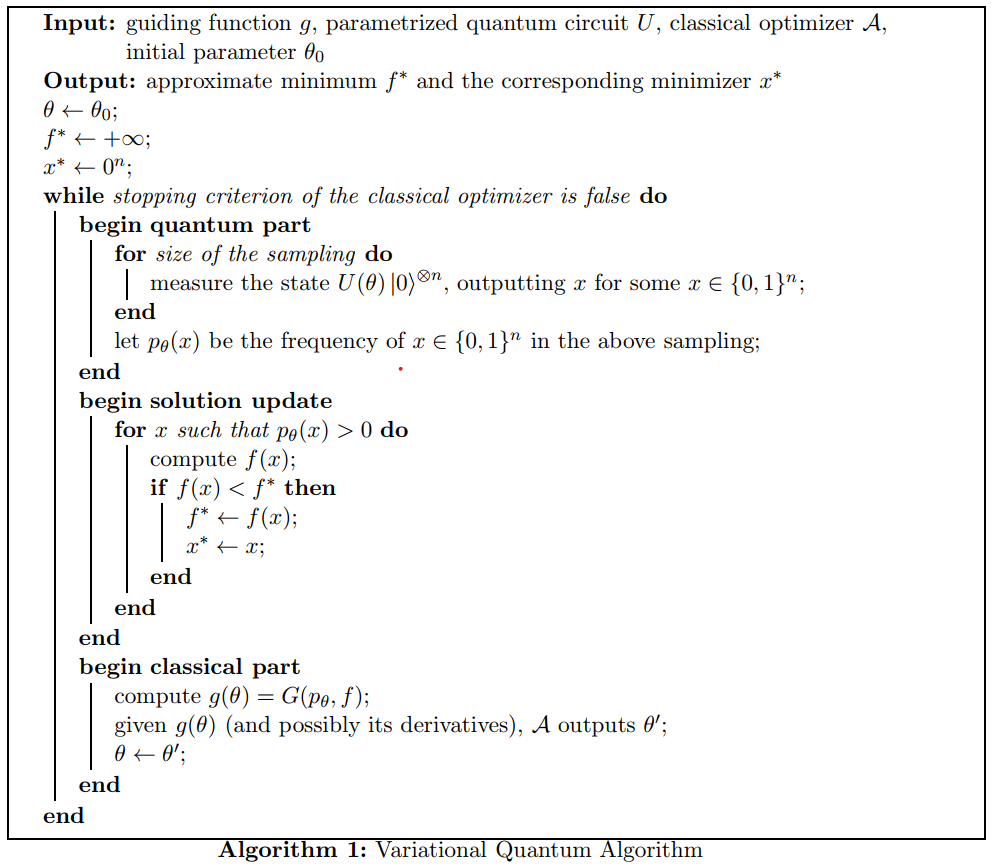
\includegraphics[width=1\linewidth]{Images/VQA-algorithm.png}
\end{figure}

The main idea of a VQA is as follows. The main loop of the algorithm executes the following steps until the classical optimizer stops according to a given stopping criterion. 

\begin{enumerate}
    \item \textbf{(Quantum part)} First, given $\theta \in \mathbb{R}^{d}$, the quantum part executes the parametrized quantum circuit $U(\theta)$ for several times to sample the quantum state. It results in a (discrete) distribution probability over $\{0,1\}^{n}$ that we note $\left\{p_{\theta}(x): x \in\{0,1\}^{n}\right\}$. % 应该是简单的频率frequency统计 % 理论上我们可以重复无数次实验,以获得该离散分布的全部信息。
    \item \textbf{(Classical part)} Second, the classical part computes the cost of this state, through the evaluation of the guiding function, according to the sampling results $p_{\theta}$, specifically, $g(\theta)=G\left(p_{\theta}, f\right)$ for a given function $G$ that is constructed from $f$ and $p_{\theta}$. For example, such $g$ can be
    \begin{equation}
    g(\theta)=\sum_{x \in\{0,1\}^n} p_\theta(x) f(x).
\end{equation}
    More precisely, for a given $\theta$, the computation of $G$ requires only the values $f(x)$ for $x$ such that $p_{\theta}(x)>0$. Eventually, this cost value is given to the classical optimizer $\mathcal{A}$, which outputs a new parameter in order to minimize $g$. % 可以用一些零阶优化技术 % Notice that, between the two parts the best-found solution is possibly updated by a classical computer.
\end{enumerate}

In the following subsections, we detail each part of VQAs and show \textbf{how specific choices of $g$ and $U$} \textbf{ensure that VQAs optimize $f$}.

\subsection{Quantum Part}

The quantum part of VQAs applies a quantum circuit on the $n$-qubit system that constitutes the quantum computer. Importantly, \textit{variational}\footnote{The word "variational" does not have that mathematical meaning.}  in VQAs stands for the parametrization of the quantum circuit. 

Let $d \in \mathbb{N}$ be the number of parameters, thus $\theta \in \mathbb{R}^d.$ A \textit{parametrized quantum circuit} is a continuous function $U: \mathbb{R}^{d} \rightarrow$ $\mathcal{M}_{2^{n}}(\mathbb{C})$ mapping any $\theta \in \mathbb{R}^{d}$ to unitary matrix $U(\theta)$.

As defined in Sect. 2.3, a quantum circuit is a sequence of universal quantum gates' compositions and/or tensor products. Thus, all coefficients of matrix $U(\theta)$ are continuous functions on $\mathbb{R}^{d}$.

\begin{example}
    A simple example of a parametrized quantum circuit for $n=3$ and $d=3$ is depicted in Fig. 6.
\begin{figure}[h]
    \centering
    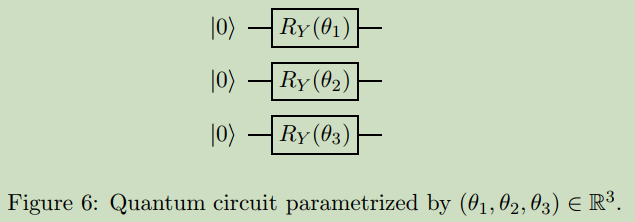
\includegraphics[width=0.75\linewidth]{Images/parametrized-quantum-circuit.png}
\end{figure}
The expression of $U(\theta)$ for this circuit is as follows: $\forall \theta=\left(\theta_1, \theta_2, \theta_3\right) \in \mathbb{R}^3$,
\begin{equation}
\begin{aligned}
& U(\theta)=R_Y\left(\theta_1\right) \otimes R_Y\left(\theta_2\right) \otimes R_Y\left(\theta_3\right) \\
& =\left(\begin{array}{cc}
\cos \frac{\theta_1}{2} & -\sin \frac{\theta_1}{2} \\
\sin \frac{\theta_1}{2} & \cos \frac{\theta_1}{2}
\end{array}\right) \otimes\left(\begin{array}{cc}
\cos \frac{\theta_2}{2} & -\sin \frac{\theta_2}{2} \\
\sin \frac{\theta_2}{2} & \cos \frac{\theta_2}{2}
\end{array}\right) \otimes\left(\begin{array}{cc}
\cos \frac{\theta_3}{2} & -\sin \frac{\theta_3}{2} \\
\sin \frac{\theta_3}{2} & \cos \frac{\theta_3}{2}
\end{array}\right) \\
& =\left(\begin{array}{cccccccc}
c_1 c_2 c_3 & -c_1 c_2 s_3 & -c_1 s_2 c_3 & c_1 s_2 s_3 & -s_1 c_2 c_3 & s_1 c_2 s_3 & s_1 s_2 c_3 & -s_1 s_2 s_3 \\
c_1 c_2 s_3 & c_1 c_2 c_3 & -c_1 s_2 s_3 & -c_1 s_2 c_3 & -s_1 c_2 s_3 & -s_1 c_2 c_3 & s_1 s_2 s_3 & s_1 s_2 c_3 \\
c_1 s_2 c_3 & -c_1 s_2 s_3 & c_1 c_2 c_3 & -c_1 c_2 s_3 & -s_1 s_2 c_3 & s_1 s_2 s_3 & -s_1 c_2 c_3 & s_1 c_2 s_3 \\
c_1 s_2 s_3 & c_1 s_2 c_3 & c_1 c_2 s_3 & c_1 c_2 c_3 & -s_1 s_2 s_3 & -s_1 s_2 c_3 & -s_1 c_2 s_3 & -s_1 c_2 c_3 \\
s_1 c_2 c_3 & -s_1 c_2 s_3 & -s_1 s_2 c_3 & s_1 s_2 s_3 & c_1 c_2 c_3 & -c_1 c_2 s_3 & -c_1 s_2 c_3 & c_1 s_2 s_3 \\
s_1 c_2 s_3 & s_1 c_2 c_3 & -s_1 s_2 s_3 & -s_1 s_2 c_3 & c_1 c_2 s_3 & c_1 c_2 c_3 & -c_1 s_2 s_3 & -c_1 s_2 c_3 \\
s_1 s_2 c_3 & -s_1 s_2 s_3 & s_1 c_2 c_3 & -s_1 c_2 s_3 & c_1 s_2 c_3 & -c_1 s_2 s_3 & c_1 c_2 c_3 & -c_1 c_2 s_3 \\
s_1 s_2 s_3 & s_1 s_2 c_3 & s_1 c_2 s_3 & s_1 c_2 c_3 & c_1 s_2 s_3 & c_1 s_2 c_3 & c_1 c_2 s_3 & c_1 c_2 c_3
\end{array}\right), \\
&
\end{aligned}
\end{equation}
where $c_i=\cos \frac{\theta_i}{2}$ and $s_i=\sin \frac{\theta_i}{2}$ for $i \in[3]$.
\end{example}

\subsection{Classical Part}

The classical part of VQAs consists of a classical optimization over the parameters $\theta \in \mathbb{R}^{d}$. 

\textbf{The classical optimizer essentially aims at finding the optimal parameters $\theta^{*}$ that lead to optimal solutions of the initial problem (1) with high probability}, specifically, such that
\begin{equation}
    \sum_{s \in \mathcal{F}}\left|\left\langle s\left|U\left(\theta^{*}\right)\right| 0_{n}\right\rangle\right|^{2} \geq 1-\epsilon \tag{10}
\end{equation}
for small $\epsilon>0$. 

\begin{remark}
    \begin{itemize}
    \item We note $\mathcal{F}$ the set of optimal solutions in problem (1). We allow $\mathcal{F}$ to contain many different optimal solutions.
    \item We note $\left|0_{n}\right\rangle$ the state $|0\rangle^{\otimes n}$ to ease the reading. Here, $0_{n}=000\dots0.$
    \item $U\left(\theta\right)| 0_{n}\rangle$ is the output state of the parametrized quantum circuit.
    \item Note that we encode each possible optimization of (1), i.e, the n-bitstring, to basis state of quantum state space.
    \item We use notation $|s\rangle$ instead of $|i\rangle$ to efficiently recall that we deal with solutions of optimization problems (1). In fact, $\mathcal{F} \subset \{0,1\}^{n}$ and we use $s$ to denote the elements of $\mathcal{F}.$
    \item In fact, we measure the output state by using the computational basis. In this paper, they are $\mathcal{C B}_{n}=\left\{|i\rangle, i \in\{0,1\}^{n}\right\}$.
    \item $\left|\left\langle s\left|U\left(\theta^*\right)\right| 0_n\right\rangle\right|^2$ is the probability with outcome $s$ after measurement. Then, $\sum_{s \in \mathcal{F}}\left|\left\langle s\left|U\left(\theta^{*}\right)\right| 0_{n}\right\rangle\right|^{2}$ is the probability with arbitrary optimal solutions after measurement.
    \end{itemize}
\end{remark}

The classical part is characterized by two aspects: 
\begin{enumerate}
    \item the function that guides the optimization
    \item the optimizer itself.
\end{enumerate}

\subsection{Guiding Function}

Let us denote 
\begin{equation}
    \mathcal{F}_{\text {quant }}=\left\{\sum_{s \in \mathcal{F}} \psi_{s}|s\rangle: \sum_{s \in \mathcal{F}}\left|\psi_{s}\right|^{2}=1\right\}
\end{equation}
as the set of quantum states that are superpositions of optimal solutions of problem (1). So if we measure any state in $\mathcal{F}_{\text {quant }}$, our result will be the optimal solution to the original optimization problem.

Let $g: \mathbb{R}^{d} \rightarrow \mathbb{R}$ be the guiding function, and $g$ acts as a link between the quantum and classical parts. \textbf{Naturally, we would like to define $g$ such that minimizing $g$ tends to minimize $f$.}

\begin{definition}[Guiding function]
    Let $g: \mathbb{R}^{d} \rightarrow \mathbb{R}$ be a function and $\mathcal{G}$ be its set of minimizers. We call $g$ \textit{a guiding function for $f$ with respect to $U$} if $g$ is continuous and
\begin{equation}
    \left\{U(\theta)\left|0_{n}\right\rangle: \theta \in \mathcal{G}\right\} \subseteq \mathcal{F}_{\text {quant}}. \tag{11}
\end{equation}
\end{definition}

\begin{itemize}
    \item Indeed, Equation (11) implies that measuring the quantum state $U\left(\theta\right)|0\rangle^{\otimes n}$ for any $\theta\in \mathcal{G}$ outputs with probability 1 an optimal solution of the initial problem $s \in \mathcal{F}$.
    \item In other words, optima of a guiding function $g$ must lead to optima of $f$ or superpositions of optima of $f$.
    \item Thus, minimizing $f$ amounts to minimizing $g$, and finding $\mathcal{F}$ is done by finding $\mathcal{G}$. The latter is found with the classical optimizer.
\end{itemize}

% 下面两个remark亟需解决!

\begin{remark}
    Without any information on $\mathcal{F}$, we need to choose a quantum circuit $U$ such that any optimal solution $s \in \mathcal{F}$ is reachable, specifically, we construct $U$ such that
\begin{equation}
    \left\{U(\theta)\left|0_{n}\right\rangle: \theta \in \mathbb{R}^{d}\right\} \supseteq \mathcal{C} \mathcal{B}_{n} \supseteq \mathcal{F}. \tag{12}
\end{equation}
Notice that this condition is weak and easily satisfied. For instance, the circuit depicted in Fig. 6 satisfies this condition. % 这段话暗示了,U的构造也需要精心设计的。
\end{remark}

\begin{remark}
If ever one is interested in finding all optimal solutions of problem (1), the circuit and the guiding function should satisfy instead the stronger condition than (11)
\begin{equation}
    \left\{U(\theta)\left|0_{n}\right\rangle: \theta \in \mathcal{G}\right\}=\mathcal{F}_{\text {quant}}. \tag{13}
\end{equation}
In that case, $U$ satisfying (12) is not enough. Without any information on $\mathcal{F}$, we need to choose $U$ that can reach any $n$-qubit quantum states, specifically, % 这段话暗示了,U的构造也需要精心设计的。
\begin{equation}
    \left\{U(\theta)\left|0_{n}\right\rangle: \theta \in \mathbb{R}^{d}\right\}=\left\{\sum_{x \in\{0,1\}^{n}} \psi_{x}|x\rangle: \sum_{x \in\{0,1\}^{n}}\left|\psi_{x}\right|^{2}=1\right\}
\end{equation}
% 上式右侧是全部整个quantum state space!
\end{remark}

\begin{definition}[Mean function]
A popular choice for the guiding function in the literature is the \textit{mean function}
\begin{equation}
    g_{\text {mean }}(\theta)=\sum_{x \in\{0,1\}^{n}} p_{\theta}(x) f(x), \tag{14}
\end{equation}
where
\begin{equation}
    p_{\theta}(x)=\left|\left\langle x|U(\theta)| 0_{n}\right\rangle\right|^{2}
\end{equation}
is the probability of finding $x$ when $U(\theta)\left|0_{n}\right\rangle$ is measured.  % 注意,此处定义中的概率p是理论上的精确概率.
\end{definition}

We find that, $\theta$ decides $U(\theta)$ (once we set up the construct of circuit); then, $\theta$ decides output state $U(\theta)\left|0_{n}\right\rangle$ (the input state is always $\left|0_{n}\right\rangle$); then, $\theta$ decides the probability distribution $\{p_{\theta}(x)\}_{x}$. On the other hand, the values of $f(x)$ are unrelated to $\theta.$ Finally, for fixed optimization problem $\min _{x \in\{0,1\}^{n}} f(x)$ and well-constructed quantum circuit $U(\theta)$, the mean function $g_{\text {mean }}(\theta)$ only is concerned about parameter $\theta.$ 

\begin{proposition}
    Function $g_{\text {mean }}$ is a guiding function.
\end{proposition}

\begin{proof}
Let us prove that $g_{\text {mean }}$ is continuous.
Let $x \in\{0,1\}^{n}$. The function $\theta \mapsto$ $p_{\theta}(x)=\left|\left\langle x|U(\theta)| 0_{n}\right\rangle\right|^{2}$ is continuous, because each coefficient of $U(\theta)$ is continuous. Thus, because multiplication and addition preserve continuity, $g_{\text {mean }}$ is continuous.

We prove by contradiction that (11) holds.
Let $\theta \in \mathcal{G}$ and let us consider the quantum state $|\psi(\theta)\rangle=U(\theta)\left|0_{n}\right\rangle$. Its decomposition in the canonical basis is $|\psi(\theta)\rangle=\sum_{x \in\{0,1\}^{n}} \psi_{x}|x\rangle$ with $\psi_{x}=\langle x|\psi(\theta)\rangle$. %牢记x是index

Assume that there exists some $\theta$ such that $|\psi(\theta)\rangle \notin \mathcal{F}_{\text {quant }}$. By definition of $\mathcal{F}_{\text {quant }}$, there exists $x_{0} \in\{0,1\}^{n}$ such that $x_{0} \notin \mathcal{F}$ and $\left|\psi_{x_{0}}\right| \neq 0$ (nonzero coefficient). Thus,
\begin{equation}
\begin{aligned}
g_{\text {mean }}(\theta) & =\sum_{x \in\{0,1\}^{n}}\left|\psi_{x}\right|^{2} f(x) \\
& =\sum_{x \in \mathcal{F}}\left|\psi_{x}\right|^{2} f(x)+\sum_{x \notin \mathcal{F}}\left|\psi_{x}\right|^{2} f(x) \\
& =\left(\sum_{x \in \mathcal{F}}\left|\psi_{x}\right|^{2}\right) f^{*}+\sum_{x \notin \mathcal{F}}\left|\psi_{x}\right|^{2} f(x)
\end{aligned}
\end{equation}
where $f^{*}$ is the optimal value of $f$, reached on $\mathcal{F}$. By definition, $f(x)>f^{*}, \forall x \notin \mathcal{F}$, and because we assume that $\left|\psi_{x_{0}}\right| \neq 0$, thus the second term of the sum is bounded below as follows: $\sum_{x \notin \mathcal{F}}\left|\psi_{x}\right|^{2} f(x)>\left(\sum_{x \notin \mathcal{F}}\left|\psi_{x}\right|^{2}\right) f^{*}$, where $\sum_{x \notin \mathcal{F}}\left|\psi_{x}\right|^{2} \geq$ $\left|\psi_{x_{0}}\right|^{2}>0$. Thus,
\begin{equation}
    g_{\text {mean }}(\theta)>\left(\sum_{x \in \mathcal{F}}\left|\psi_{x}\right|^{2}\right) f^{*}+\left(\sum_{x \notin \mathcal{F}}\left|\psi_{x}\right|^{2}\right) f^{*}=f^{*}
\end{equation}
This contradicts the previous statement that $\theta \in \mathcal{G}$, as one readily verifies that the infimum of $g_{\text {mean }}$ is $g_{\text {mean }}^{*}=f^{*}$.
% 这来自于一个简单的命题。考虑一些实数的凸组合(系数非负且和为一),那么它们组合的结果的上限是这些实数中的最大值,其下限是这些实数中的最小值。
\end{proof}

\begin{example}
    We illustrate the mean function on the 3-qubit quantum circuit $U(\theta)$ depicted in Fig. 6. The single application of rotation gate $R_{Y}$ in Eq. (6) of angle $\theta_{i}$ on a qubit initially on state $|0\rangle$ is
\begin{equation}
\begin{aligned}
R_{Y}\left(\theta_{i}\right)|0\rangle & =\cos \frac{\theta_{i}}{2}|0\rangle+\sin \frac{\theta_{i}}{2}|1\rangle \\
& =\sum_{j \in\{0,1\}} \cos \frac{\theta_{i}-j \pi}{2}|j\rangle
\end{aligned}
\end{equation}
since $\sin (\phi)=\cos \left(\phi-\frac{\pi}{2}\right)$ for any $\phi \in \mathbb{R}$. Eventually, the quantum state resulting from $U(\theta)$ is
\begin{equation}
\begin{aligned}
U(\theta)\left|0_{3}\right\rangle & =\bigotimes_{i=1}^{3} R_{Y, i}\left(\theta_{i}\right)|0\rangle \\
& =\sum_{j_{1}, j_{2}, j_{3} \in\{0,1\}}\left(\prod_{i=1}^{3} \cos \frac{\theta_{i}-j_{i} \pi}{2}\right)\left|j_{1} j_{2} j_{3}\right\rangle.
\end{aligned}
\end{equation}
Thus, the probability to measure $x=\left(x_{1}, x_{2}, x_{3}\right) \in\{0,1\}^{3}$ is
\begin{equation}
    p_{\theta}(x)=\left(\prod_{i=1}^{3} \cos \frac{\theta_{i}-x_{i} \pi}{2}\right)^{2} \tag{15}
\end{equation}
and the expression of $g_{\text {mean }}$ of equation (14) directly results from it.
\end{example}

\subsection{Classical Optimizer} % 需要复习一下概率论,请先阅读

The role of the classical optimizer is to minimize the guiding function. The function $g$ is continuous and is usually differentiable but \textit{not convex}. Any unconstrained optimization algorithm can be used to minimize $g$.

\textbf{To speak in terms of stochastic optimization}, the classical optimizer aims at solving the stochastic programming model under \textit{endogenous uncertainty} 
\begin{equation}
    \min _{\theta}\left\{g(\theta)=\mathbb{E}_{\xi_{\theta} \sim p_{\theta}}\left[G\left(\theta, \xi_{\theta}\right)\right]\right\} \tag{19}
\end{equation}
where the definition of $G$ depends on the choice of a specific guiding function $g$, and $\xi_{\theta}$ is an endogenous random variable that depends on $\theta$. Specifically, $\xi_{\theta}$ is a discrete random variable, with the set of possible outcomes $\{0,1\}^{n}$ and the following distribution probability:
\begin{equation}
    \mathbb{P}\left(\xi_{\theta}=x\right)=p_{\theta}(x), \quad \forall x \in\{0,1\}^{n}.
\end{equation}
\begin{example}
    For instance, for the case of $g=g_{\text {mean }}$, we have
\begin{equation}
    G\left(\theta, \xi_{\theta}\right)=f\left(\xi_{\theta}\right).
\end{equation}
Then, 
\begin{equation}
    g_{\text {mean }}(\theta)
=\mathbb{E}_{\xi_{\theta} \sim p_{\theta}}\left[f\left(\xi_{\theta}\right)\right]
=\sum_{x \in\{0,1\}^{n}} p_{\theta}(x) f(x).
\end{equation}
\end{example}

\todo{How to consider the another guiding function --- Gibbs function?}

The problem (19) falls into the class of \textbf{stochastic dependent-decision probabilities problems}. % 目前的理解是,在式(19)中,theta决定了随机变量xi_theta,通过期望的计算消除了该随机变量的随机性。但外从外部看,其整体是依赖于变量theta。
In practice, the classical optimizer approximates the value of objective function $g(\theta)$ by a \textit{Monte Carlo estimation} as follows:
\begin{equation}
    \hat{g}_{N}(\theta)=\frac{1}{N} \sum_{j=1}^{N} G\left(\theta, \xi_{\theta}^{j}\right)
\end{equation}
where $\left\{\xi_{\theta}^{j}\right\}_{j \in[N]}$ is a sample of size $N$ from the distribution of $\xi_{\theta}$. Notice that for a given $\theta$, the quantity $\hat{g}_{N}(\theta)$ itself is a random variable since its value depends on the sample that has been generated, which is random. In contrast, the value of $g(\theta)$ is deterministic. Notice that according to the Law of Large Numbers, $\hat{g}_{N}(\theta)$ converges with probability one to $g(\theta)$ as $N \rightarrow \infty$.

\begin{example}
For instance, for the case of $g=g_{\text {mean }}$, we have
\begin{equation}
    G\left(\theta, \xi_{\theta}\right)=f\left(\xi_{\theta}\right)
\end{equation}
Hence, for each $\xi_{\theta}^{j} \in\{0,1\}^{n}$ sampled, either we compute classically $f(\xi_{\theta}^{j})$ and store it if not already computed, or we get its value. Thus, we can compute $\hat{g}_{N}(\theta)$. 
\end{example}

\section{Quantum Approximate Optimization Algorithm}

In this section, we consider optimization problems of the form
\begin{equation}
    \min _{x \in\{0,1\}^n} f(x), \tag{1}
\end{equation}
where $f$ is any function defined on $\{0,1\}^n$. We assume throughout this section that the function $f$ is \textit{polynomial}. Since $x$ is a binary variable,  we can write
\begin{align}
    f(x)&=\sum_{i_1=0}^1 \sum_{i_2=0}^1 \cdots \sum_{i_n=0}^1 a_{i_1 i_2 \cdots i_n} x_1^{i_1} x_2^{i_2} \cdots x_n^{i_n}\\
    &=\sum_{i=\left(i_1, \ldots ,i_n\right) \in\{0,1\}^n} a_i \prod_{k=1}^n x_k^{i_k}.
\end{align}
For example, in case of two variables:
\begin{equation}
    f(x, y)=\sum_{i=0}^1 \sum_{j=0}^1 a_{i j} x^i y^j=a_{00}+a_{10} x+a_{01} y+a_{11} x y.
\end{equation}

First, we reformulate problem (1) to a more suitable form for quantum optimization. This reformulation is motivated by the \textit{quantum adiabatic evolution} that, for a given Hermitian matrix, approximates the eigenvector with the lowest eigenvalue under certain conditions. 

For that, we interpret the objective function of problem (1) as a $2^n$ by $2^n$ diagonal Hermitian matrix $H_{f}$ such that each eigenvector $\left|u_{x}\right\rangle$ is matching a classical solution $x \in\{0,1\}^{n}$ with an eigenvalue equal to $f(x)$, specifically,
\begin{equation}
    H_{f}\left|u_{x}\right\rangle=f(x)\left|u_{x}\right\rangle .
\end{equation}
\textbf{Thus, the solutions of problem (1) are the solutions corresponding to the lowest eigenvalues of $H_{f}$.} \textbf{The Quantum Approximate Optimization Algorithm (QAOA) presented in this section aims at finding the lowest eigenvalue of $H_{f}$.} % 本节概括

\subsection{Problem Reformulation}

The construction of $H_{f}$ is as follows. 

(1) First, we transform the $\{0,1\}$ problem (1) into a $\{-1,1\}$ problem. For that, we apply the following linear transformation: for $x=$ $\left(x_{1}, \ldots, x_{n}\right) \in\{0,1\}^{n}$, we define $z=\left(z_{1}, \ldots, z_{n}\right) \in\{-1,1\}^{n}$ where
\begin{equation}
    z_{i}=1-2 x_{i}, \forall i \in[n]. \tag{20}
\end{equation}
(Note that $x_{i}=0$ iff $z_i=1$, and $x_{i}=1$ iff $z_i=-1.$) This leads to the problem
\begin{equation}
    \min _{z \in\{-1,1\}^{n}} f_{ \pm}(z)
\end{equation}
where, for $z \in\{-1,1\}^{n}$,
\begin{equation}
    f_{ \pm}(z)=\sum_{\alpha=\left(\alpha_{1}, \ldots \alpha_{n}\right) \in\{0,1\}^{n}} h_{\alpha} \prod_{i=1}^{n} z_{i}^{\alpha_{i}}
\end{equation}
where $h_{\alpha} \in \mathbb{R}, \forall \alpha \in\{0,1\}^{n}$. Recall that we assumed $f$ to be \textit{multilinear polynomial}. % 通过(20)这样子简单的换元操作,multilinear polynomial在数学形式上是不变的。

(2) Second, we define the $2^n$ by $2^n$ matrix $H_{f}$ (called "Hamiltonian") as
\begin{equation}
    H_{f}:=\sum_{\alpha=\left(\alpha_{1}, \ldots \alpha_{n}\right) \in\{0,1\}^{n}} h_{\alpha} \bigotimes_{i=1}^{n} Z_{i}^{\alpha_{i}}
\end{equation}
where $Z=\left(\begin{array}{cc}1 & 0 \\ 0 & -1\end{array}\right), Z^{0}=I$ and $Z^{1}=Z$. \textbf{We note $Z_{i}$ the application of $Z$ to qubit $i$. } % number z --> gate Z; product --> tensor product

\begin{itemize}
    \item Note that the tensor product of Hermitian matrices is also Hermitian, and the $\mathbb{R}$-linear combination of Hermitian matrices is again Hermitian. Hence, $H_{f}$ above is Hermitian.
    \item Notice that $Z$ is equal to the universal gate $R_{Z}(\pi)$ modulo a global phase (see Eq. (7)).
\end{itemize}

This construction of $H_{f}$ leads to the following property.

\begin{proposition}
    The eigenvectors of $H_{f}$ are the canonical basis $|x\rangle \in \mathcal{C B}_{n}$ with eigenvalues that are the cost of the solutions $f(x)$, specifically,
\begin{equation}
    \forall|x\rangle \in \mathcal{C B}_{n}, \quad H_{f}|x\rangle=f(x)|x\rangle. \tag{21}
\end{equation}
\end{proposition}
\begin{proof}
    First, the eigenvectors of $H_{f}$ are the canonical basis states. Indeed, each term of the sum that constitutes $H_{f}$ is a tensor product of $n$ matrices $I$ or $Z$, both diagonal\footnote{The tensor product of two diagonal matrices is also diagonal}. Thus, $H_{f}$ is a $2^{n}$ diagonal matrix. 

    Second, let us find the eigenvalues associated with the eigenvectors. Let $|x\rangle=\left|x_{1} \ldots x_{n}\right\rangle$ be in $\mathcal{C B}_{n}$. Let $z=\left(z_{1}, \ldots, z_{n}\right)$ be the result of transformation (20). Thus, we can easily show that 
\begin{equation}
    Z^{0}\left|x_{i}\right\rangle=I\left|x_{i}\right\rangle=z_{i}^{0}\left|x_{i}\right\rangle,Z^{1}\left|x_{i}\right\rangle=Z\left|x_{i}\right\rangle=z_{i}^{1}\left|x_{i}\right\rangle, \forall i \in[n],
\end{equation}
and
\begin{equation}
\begin{aligned}
H_{f}|x\rangle 
& =\left(\sum_{\alpha=\left(\alpha_{1}, \ldots \alpha_{n}\right) \in\{0,1\}^{n}} h_{\alpha} \bigotimes_{i=1}^{n} Z_{i}^{\alpha_{i}}\right) \left|x_{1} \ldots x_{n}\right\rangle\\
& =\sum_{\alpha=\left(\alpha_{1}, \ldots \alpha_{n}\right) \in\{0,1\}^{n}} h_{\alpha} \left(\bigotimes_{i=1}^{n} Z_{i}^{\alpha_{i}}\right) \left|x_{1} \ldots x_{n}\right\rangle\\
& =\sum_{\alpha=\left(\alpha_{1}, \ldots, \alpha_{n}\right) \in\{0,1\}^{n}} h_{\alpha} \left( \bigotimes_{i=1}^{n} Z_{i}^{\alpha_{i}}\left|x_{i}\right\rangle\right) \\
& =\sum_{\alpha=\left(\alpha_{1}, \ldots, \alpha_{n}\right) \in\{0,1\}^{n}} h_{\alpha} \left(\bigotimes_{i=1}^{n} z_{i}^{\alpha_{i}}\left|x_{i}\right\rangle\right) \\
& =\sum_{\alpha=\left(\alpha_{1}, \ldots, \alpha_{n}\right) \in\{0,1\}^{n}} h_{\alpha} \left(\prod_{i=1}^{n} z_{i}^{\alpha_{i}}\left|x_{i}\right\rangle\right) \\
& =\sum_{\alpha=\left(\alpha_{1}, \ldots \alpha_{n}\right) \in\{0,1\}^{n}} h_{\alpha} \left(\prod_{i=1}^{n} z_{i}^{\alpha_{i}}\right) \left|x_{1} \ldots x_{n}\right\rangle\\
& =\left(\sum_{\alpha=\left(\alpha_{1}, \ldots, \alpha_{n}\right) \in\{0,1\}^{n}} h_{\alpha} \prod_{i=1}^{n} z_{i}^{\alpha_{i}}\right)|x\rangle \\
& =f_{ \pm}(z)|x\rangle \\
& =f(x)|x\rangle .
\end{aligned}
\end{equation}
\end{proof}
\begin{example}
    We illustrate this transformation on a small example with $n=2$. Let us consider the problem
\begin{equation}
    \min _{x \in\{0,1\}^{2}} f(x)=x_{1}+2 x_{2}-3 x_{1} x_{2}.
\end{equation}
Using (20), the equivalent $\{-1,1\}$-problem is
\begin{equation}
    \min _{z \in\{-1,1\}^{2}} f_{ \pm}(z)=\frac{1}{4} z_{1}-\frac{1}{4} z_{2}-\frac{3}{4} z_{1} z_{2}+\frac{3}{4}.
\end{equation}
Thus, the Hermitian matrix associated with the problem is
\begin{equation}
    H_{f}=\frac{1}{4} Z \otimes I-\frac{1}{4} I \otimes Z-\frac{3}{4} Z \otimes Z+\frac{3}{4} I \otimes I
\end{equation}
To illustrate (21), we compute the eigenvalue of the canonical basis state $|10\rangle$.
\begin{equation}
\begin{aligned}
H_{f}|10\rangle & =\frac{1}{4}(Z \otimes I)|10\rangle-\frac{1}{4}(I \otimes Z)|10\rangle-\frac{3}{4}(Z \otimes Z)|10\rangle+\frac{3}{4}(I \otimes I)|10\rangle \\
& =-\frac{1}{4}|10\rangle-\frac{1}{4}|10\rangle+\frac{3}{4}|10\rangle+\frac{3}{4}|10\rangle \\
& =|10\rangle \\
& =f(1,0)|10\rangle
\end{aligned}
\end{equation}
because $f(1,0)=1$.
\end{example}

Notice that most of the problems solved with QAOA in the literature are QUBO (Quadratic Unconstrained Binary Optimization) problems. Thus, $H_{f}$ has the specific form
\begin{equation}
    H_{f}=\sum_{i} h_{i i} Z_{i}+\sum_{i<j} h_{i j} Z_{i} \otimes Z_{j}
\end{equation}
where $h_{i j} \in \mathbb{R}, \forall i \leq j$. Note that $Z_{i}$ the application of $Z$ to qubit $i$. As mentioned before, we use the notation $Z_{i}$ for the application of $Z$ on qubit $i$ (and the application of identity matrix on the remaining qubits). Like in Example 33, $Z_1=Z \otimes I$ and $Z_2=I \otimes Z$.

\begin{remark}
    It is justified by the fact that solving QUBO problems to optimality is already NP-hard, and the quantum gates of the circuit are easier to implement on hardware in that case.

\href{https://ww2.mathworks.cn/help/matlab/math/what-is-a-qubo.html}{What is a QUBO Problem? - MATLAB \& Simulink - MathWorks} 
\end{remark}

\subsection{Quantum Part}

QAOA is a Variational Quantum Algorithm where the quantum part derives from the Hamiltonian $H_{f}$. This quantum part consists of a quantum circuit with $2 p$ parameters $(\boldsymbol{\gamma}, \boldsymbol{\beta})=\left(\gamma_{1}, \ldots, \gamma_{p}, \beta_{1}, \ldots, \beta_{p}\right) \in \mathbb{R}^{2 p}$, where $p$ is called \textit{depth}. 

\begin{definition}[Unitary operator associated with Hermitian matrix]
    Given a Hermitian matrix $A$, we define its associated quantum gate $\operatorname{Exp}(A, t)$ parametrized by the parameter $t \in \mathbb{R}$ as:
\begin{equation}
    \operatorname{Exp}(A, t) =e^{-i A t} 
=\sum_{k=0}^{\infty} \frac{1}{k!}(-i)^{k} t^{k} A^{k}.
\end{equation}
Because $A$ is Hermitian, $\operatorname{Exp}(A, t)$ is a unitary matrix.
\end{definition}

The quantum circuit $U(\boldsymbol{\gamma}, \boldsymbol{\beta})$ is the sequence of $p$ layers of two blocks, initially applied to the uniform superposition $|+\rangle^{\otimes n}$. %意思就是两个一组,一共有p组在一起。
\begin{itemize}
    \item The first block is of the form $\operatorname{Exp}\left(H_{f}, \gamma\right)$, for $\gamma \in \mathbb{R}$, which is the unitary operator associated with the Hamiltonian $H_{f}$.
    \item The second block is of the form $\operatorname{Exp}\left(H_{B}, \beta\right)$, for $\beta \in \mathbb{R}$, which is the unitary operator associated with the Hamiltonian
    \begin{equation}
    H_{B}=\sum_{i=1}^{n} R_{X, i}(\pi).
\end{equation}
\end{itemize}
Thus, the quantum circuit is
\begin{equation}
    U(\boldsymbol{\gamma}, \boldsymbol{\beta})=\operatorname{Exp}\left(H_{B}, \beta_{p}\right) \operatorname{Exp}\left(H_{f}, \gamma_{p}\right) \ldots \operatorname{Exp}\left(H_{B}, \beta_{1}\right) \operatorname{Exp}\left(H_{f}, \gamma_{1}\right) H^{\otimes n} \tag{22}
\end{equation}
where the first gates applied in this circuit are $H^{\otimes n}$m, to then apply the $p$ layers to state $|+\rangle^{\otimes n}$. 

The three propositions that follow express the quantum circuit of QAOA with the set of universal gates (see Theorem 13). We give first the general decomposition of the QAOA quantum circuit defined in (22).

\begin{proposition}
    The first block $\operatorname{Exp}\left(H_{f}, \gamma\right)$ parametrized by $\gamma \in \mathbb{R}$ is
\begin{equation}
    \operatorname{Exp}\left(H_{f}, \gamma\right)=\prod_{\alpha \in\{0,1\}^{n}} \operatorname{Exp}\left(\bigotimes_{i=1}^{n} Z_{i}^{\alpha_{i}}, h_{\alpha} \gamma\right)
\end{equation}
The second block $\operatorname{Exp}\left(H_{B}, \beta\right)$ parametrized by $\beta \in \mathbb{R}$ is
\begin{equation}
    \operatorname{Exp}\left(H_{B}, \beta\right)=\bigotimes_{i=1}^{n} R_{X, i}(2 \beta)
\end{equation}
\end{proposition}

\begin{remark}
    The Kronecker sum satisfies the nice property
\begin{equation}
    \exp (A) \otimes \exp (B)=\exp (A \oplus B)
\end{equation}
(Horn and Johnson 1994, p. 208).
\begin{equation}
    e^{\mathrm{A}} e^{\mathrm{B}}=e^{\mathrm{A}+\mathrm{B}}
\end{equation}
holds only when $A$ and $B$ commute, i.e.,$[A, B]=A B-B A=0.$
\end{remark}

\begin{proof}
Let $\gamma \in \mathbb{R}$ and let us consider the first block $\operatorname{Exp}\left(H_{f}, \gamma\right)$. By Definition 43, and because each pair of matrices of the family $\left\{\bigotimes_{i=1}^{n} Z_{i}^{\alpha_{i}}: \alpha=\left(\alpha_{1}, \ldots, \alpha_{n}\right) \in\{0,1\}^{n}\right\}$ commutes two by two, %two by two 两个一组地
\begin{align}
\operatorname{Exp}\left(H_{f}, \gamma\right) & =e^{-i\left(\sum_{\alpha=\left(\alpha_{1}, \ldots, \alpha_{n}\right) \in(0,1)^{n}} h_{\alpha} \bigotimes_{i=1}^{n} Z_{i}^{\alpha_{i}}\right) \gamma}  \tag{23}\\
& =\prod_{\alpha=\left(\alpha_{1}, \ldots, \alpha_{n}\right) \in\{0,1\}^{n}} e^{-i h_{\alpha} \bigotimes_{i=1}^{n} Z_{i}^{\alpha_{i}} \gamma}  \tag{24}\\
& =\prod_{\alpha=\left(\alpha_{1}, \ldots, \alpha_{n}\right) \in\{0,1\}^{n}} \operatorname{Exp}\left(\bigotimes_{i=1}^{n} Z_{i}^{\alpha_{i}}, h_{\alpha} \gamma\right). \tag{25}
\end{align}

Let $\beta \in \mathbb{R}$ and let us consider the second block $\operatorname{Exp}\left(H_{B}, \beta\right)$. For more readability, we write $X_{i}=R_{X, i}(\pi)$, the application of matrix $X=\left(\begin{array}{ll}0 & 1 \\ 1 & 0\end{array}\right)$ on qubit $i$. With the same development as above, and because each pair of matrices of the family $\left\{X_{i}: i \in[n]\right\}$ commutes two by two,
\begin{equation}
    \operatorname{Exp}\left(H_{B}, \beta\right)=\prod_{i=1}^{n} \operatorname{Exp}\left(X_{i}, \beta\right)
\end{equation}
Let $i \in[n]$. Thus,
\begin{align}
\operatorname{Exp}\left(X_{i}, \beta\right) & =\sum_{k=0}^{\infty} \frac{1}{k!}(-i)^{k} \beta^{k} X_{i}^{k}  \tag{26}\\
& =\sum_{k=0}^{\infty} \frac{1}{(2 k)!}(-i)^{2 k} \beta^{2 k} X_{i}^{2 k}+\sum_{k=0}^{\infty} \frac{1}{(2 k+1)!}(-i)^{(2 k+1)} \beta^{(2 k+1)} X_{i}^{(2 k+1)} \tag{27} \\
& =\sum_{k=0}^{\infty} \frac{1}{(2 k)!}(-i)^{2 k} \beta^{2 k} I+\sum_{k=0}^{\infty} \frac{1}{(2 k+1)!}(-i)^{(2 k+1)} \beta^{(2 k+1)} X_{i}  \tag{28}\\
& =\sum_{k=0}^{\infty} \frac{1}{(2 k)!}(-1)^{k} \beta^{2 k} I-i \sum_{k=0}^{\infty} \frac{1}{(2 k+1)!}(-1)^{k} \beta^{(2 k+1)} X_{i}  \tag{29}\\
& =\cos (\beta) I-i \sin (\beta) X_{i}  \tag{30}\\
& =R_{X, i}(2 \beta) \tag{31}
\end{align}
where line (28) exploits the fact that $X^{2}=I$, implying $X^{2 k}=I$ and $X^{2 k+1}=X$. Moreover, line (29) applies the definition of the complex number $i$, and one can recognize the power series of cosines and sinus functions.
\end{proof}

The particular case of QUBO is mainly considered in the literature. 

Thus, we propose next a decomposition of the QAOA quantum circuit for this specific case, see Appendix B.2.2 for a proof.

\begin{proposition}
    For the case of QUBO, the expression of $\operatorname{Exp}\left(H_{f}, \gamma\right)$ simplifies in
\begin{equation}
    \operatorname{Exp}\left(H_{f}, \gamma\right)=\left(\bigotimes_{i=1}^{n} R_{Z, i}\left(2 h_{i i} \gamma\right)\right) \prod_{i<j} C X_{i, j} R_{Z, j}\left(2 h_{i, j} \gamma\right) C X_{i, j}
\end{equation}
and is rather easily implemented with universal quantum gates.
\end{proposition}

\begin{proof}
    Proof Let $\gamma \in \mathbb{R}$. The application of (23)-(25) to the case of QUBO gives
\begin{equation}
\begin{aligned}
\operatorname{Exp}\left(H_{f}, \gamma\right) & =e^{-i\left(\sum_{i=1}^{n} h_{i i} Z_{i}+\sum_{i<j} h_{i j} Z_{i} \otimes Z_{j}\right) \gamma} \\
& =\prod_{i=1}^{n} e^{-i Z_{i} h_{i i} \gamma} \prod_{i<j} e^{-i Z_{i} \otimes Z_{j} h_{i j} \gamma} \\
& =\prod_{i=1}^{n} \operatorname{Exp}\left(Z_{i}, h_{i i} \gamma\right) \prod_{i<j} \operatorname{Exp}\left(Z_{i} \otimes Z_{j}, h_{i j} \gamma\right)
\end{aligned}
\end{equation}
Then, let us prove that, for $i \in[n]$ and $t \in \mathbb{R}, \operatorname{Exp}\left(Z_{i}, t\right)=R_{Z, i}(2 t)$. The same development as above (28)-(30), replacing $X$ by $Z$ that have the same property $Z^{2}=I$, gives
\begin{align}
\operatorname{Exp}\left(Z_{i}, t\right) & =\cos (t) I-i \sin (t) Z_{i}  \tag{32}\\
& =R_{Z, i}(2 t) \tag{33}
\end{align}
Eventually, line (32) is the application of the gate $\left(\begin{array}{cc}e^{-i t} & 0 \\ 0 & e^{i t}\end{array}\right)=R_{Z}(2 t)$ on qubit $i$, and the identity on the others.

It remains to prove that, for $i<j \in[n]$ and $t \in \mathbb{R}, \operatorname{Exp}\left(Z_{i} \otimes Z_{j}, t\right)=$ $C X_{i, j} R_{Z, j}(2 t) C X_{i, j}$. Following the same developments as above, we have
\begin{equation}
    \operatorname{Exp}\left(Z_{i} \otimes Z_{j}, t\right)=\cos (t) I-i \sin (t) Z_{i} \otimes Z_{j} \tag{34}
\end{equation}
We consider the two-qubit system that corresponds to the qubit $i$ as the first qubit and the qubit $j$ as the second qubit (the others are unchanged by the transformation). Thus, it remains to prove the equality of the two circuits depicted on Fig. 9.
\begin{figure}[h]
    \centering
    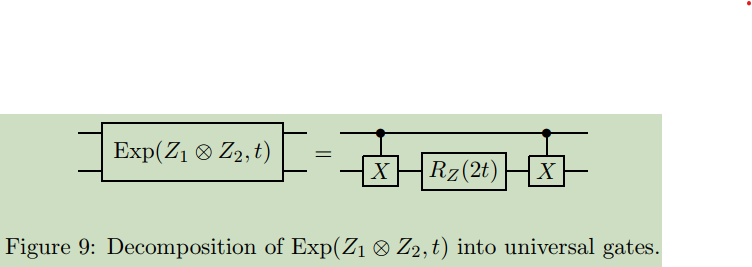
\includegraphics[width=0.75\linewidth]{Images/grange23-f9.png}
\end{figure}
On the one hand, (34) is the application of the gate $=\left(\begin{array}{cc}R_{Z}(2 t) & 0 \\ 0 & R_{Z}(-2 t)\end{array}\right)$ to this system. Indeed,

\begin{equation}
\begin{aligned}
\cos (t) I-i \sin (t) Z_{1} \otimes Z_{2} & =\cos (t)\left(\begin{array}{llll}
1 & 0 & 0 & 0 \\
0 & 1 & 0 & 0 \\
0 & 0 & 1 & 0 \\
0 & 0 & 0 & 1
\end{array}\right)-i \sin (t)\left(\begin{array}{cccc}
1 & 0 & 0 & 0 \\
0 & -1 & 0 & 0 \\
0 & 0 & -1 & 0 \\
0 & 0 & 0 & 1
\end{array}\right) \\
& =\left(\begin{array}{cccc}
e^{-i t} & 0 & 0 & 0 \\
0 & e^{i t} & 0 & 0 \\
0 & 0 & e^{i t} & 0 \\
0 & 0 & 0 & e^{-i t}
\end{array}\right) \\
& =\left(\begin{array}{ccc}
R_{Z}(2 t) & 0 & \\
0 & R_{Z}(-2 t)
\end{array}\right) .
\end{aligned}
\end{equation}

On the other hand, the composition of gates $C X_{1,2} R_{Z, 2}(2 t) C X_{1,2}$ on this system amounts to
\begin{equation}
\begin{aligned}
C X_{1,2} R_{Z, 2}(2 t) C X_{1,2} & =\left(\begin{array}{cc}
I & 0 \\
0 & X
\end{array}\right)\left(\begin{array}{cc}
R_{Z}(2 t) & 0 \\
0 & R_{Z}(2 t)
\end{array}\right)\left(\begin{array}{ll}
I & 0 \\
0 & X
\end{array}\right) \\
& =\left(\begin{array}{cc}
R_{Z}(2 t) & 0 \\
0 & X R_{Z}(2 t) X
\end{array}\right) \\
& =\left(\begin{array}{cc}
R_{Z}(2 t) & 0 \\
0 & R_{Z}(-2 t)
\end{array}\right) .
\end{aligned}
\end{equation}
Thus, the proof results from replacing $t$ by appropriate values $h_{i i} \gamma$ for $i \in[n]$ and $h_{i j} \gamma$ for $i<j$.
\end{proof}

The decomposition in universal quantum gates of the term $\operatorname{Exp}\left(Z_{i} \otimes Z_{j}, t\right)$ for the specific case of QUBO (see Proposition 35) is mainly used in the literature. 
